\documentclass[11pt]{article}
\usepackage[a4paper,margin=25mm]{geometry}
\usepackage[T1]{fontenc}
\usepackage[utf8]{inputenc}
\usepackage{lmodern}
\usepackage{graphicx}
\usepackage{booktabs}
\usepackage{amsmath}
\usepackage{xspace}
\usepackage{url}
\usepackage{hyperref}
\graphicspath{{../../fullsim_analysis/results/calib/citiroc/}}
\newcommand{\us}{\textmu s\xspace}
\newcommand{\Vov}{\ensuremath{V_{\rm ov}}\xspace}

\title{Calibration of the Citiroc~1A on the dark counts of the SiPMs:\\
room temperature and two cooled scenarios\\[4pt]
\large Preliminary}
\author{J.\,J.~Gómez-Cadenas}
\date{21 October 2026}

\begin{document}
\maketitle

\begin{abstract}
The gain of each channel of the Citiroc~1A, in ADC counts per
photoelectron, is to be measured on the bench from the dark counts of the
SiPMs, with the periodic trigger of the board and the peak detector of the
chip: each trigger opens a window of fixed length, and every channel stores
the maximum of its high-gain shaped signal within it. We study this
procedure on the simulation, where the true gain of every channel is
known, in three operating scenarios. At room temperature the dark rate of
the $6 \times 6$~mm$^2$ SiPMs, about 4.4~MHz per channel, puts a pulse on
the tail of an earlier one in half of the windows; the spectrum shows
steps rather than peaks and the fitted gain is biased by 1 to 27\% in a way
that depends on the shaping and on the sample, so that the calibration
appears impracticable. Cooling the SiPMs alone to $-3~^\circ$C, with the
crystal at room temperature, reduces the dark rate to 750~kHz and the
overlapping windows to 4\%: the photoelectron peaks are clean and, at the
longest shaping of the high gain, the fitted gain of each of the 64
channels is within 1\% of the true one. Cooling the whole system to $-23~^\circ$C, a condition attractive for
BGO, reduces the dark rate to 160~kHz and the overlapping windows to
0.3\%, and gives the gain to better than 1\%, at the cost of about a
million triggers per measurement. These results use the dark-rate law of
the model; the measured temperature dependence of the same SiPM supports
them at $-23~^\circ$C for any of the published laws.
\end{abstract}

\tableofcontents

\section{Introduction}

The energy measured by the Citiroc~1A is the low-gain stored value of each
channel converted to photoelectrons, and the conversion requires the gain
of every channel in ADC counts per photoelectron and the level that a
channel with no signal stores, its zero. The SiPMs provide a calibration
source without any light: their dark avalanches, single photoelectrons
with their crosstalk companions, whose spectrum on the high-gain path is a
ladder of peaks spaced by one gain. The low-gain path follows from the
high-gain one through the ratio of the two paths, measured by charge
injection, and is not discussed here.

The bench measures this spectrum with the periodic trigger of the A5202
board and the peak detector of the chip (peak stretch): the trigger opens
a window whose length is the hold delay, and every channel stores the
maximum of its high-gain shaped signal within the window. Since the
trigger does not depend on the signal, the windows sample the dark counts
without any selection, and the measurement does not depend on the
latency of the board or on the discriminator thresholds.

The difficulty is the dark rate itself. At room temperature a
$6 \times 6$~mm$^2$ cell of the S14160 family fires several million times
per second, and the shaped pulse of each avalanche lasts a few hundred
nanoseconds; a window of 200~ns then rarely contains an isolated avalanche.
Cooling reduces the rate by about a factor of two every 9~K. We consider
three scenarios: the whole system at room temperature, 20~$^\circ$C; the
SiPMs cooled to $-3~^\circ$C by a Peltier element while the crystal stays
at room temperature; and the whole system, crystal included, at
$-23~^\circ$C (250~K), where BGO gives 1.7 times more light with a decay
time of 0.84~\us instead of 0.44~\us. The overvoltage is 5~V in the three
cases, the bias following the breakdown voltage (42.83, 42.05 and
41.37~V). The question of this note is in which of these scenarios the
calibration works, and with which settings.

\section{The measurement and its simulation}
\label{sec:method}

The simulation generates the dark avalanches of each channel from the
model of the SiPM (design document of the simulation): the dark rate at
the temperature and overvoltage of the run, each avalanche with its
crosstalk cells (19.5\% probability of at least one extra cell at 5~V) and
afterpulses, the current pulse of one avalanche across the 50~$\Omega$
input (peak at 69~ns, 100~ns fall). The Citiroc chain amplifies this
pulse with its voltage preamplifier, shapes it with the slow CR-RC$^2$
shaper of the high-gain path at the chosen peaking time (25, 50 or
87.5~ns), and adds white noise shaped the same way, 0.1~photoelectron rms
at 87.5~ns and growing as the inverse square root of the peaking time
(0.19~photoelectron at 25~ns). The output of the chain is expressed in
units of the peak of one avalanche, so that one photoelectron is one gain
of 10~ADC counts, on a pedestal of 200~counts.

The periodic trigger is emulated by windows of 200~ns opened at fixed
times along records of 6.2~\us, separated by two peaking times so that the
noise of consecutive windows is independent; in each window every channel
stores the maximum of its high-gain signal. A dark avalanche reaches the
maximum of its shaped signal 45~ns after it fires at 25~ns of peaking time
and 104~ns after at 87.5~ns, so that a window of 200~ns contains the full
pulse of an avalanche that arrives in its first half or more.

The zero of the ladder is the pedestal, the value stored with no signal
and no noise, measured on the bench with the SiPMs below breakdown
(menu~1 of the bench programme): the voltage preamplifiers of the Citiroc
pass no constant current, and the mean dark current leaves no offset.
Two estimators of the gain are compared with the true gain of each
channel. The first fits the ladder: it locates the peaks as the minima of
the smoothed second derivative of the spectrum, numbers them from the
pedestal and takes the gain as the slope of the straight line through the
first three. The second takes the position of the one-photoelectron peak
above the pedestal, fitted with a Gaussian on a linear background. Their
ratios to the true gain are written $k$ and $k_1$; both would be one for an
ideal spectrum.

\section{Room temperature: why it fails}
\label{sec:warm}

At 20~$^\circ$C and 5~V the model gives 4.4~MHz per channel, close to the
4.5~MHz measured by POLAR-2 on the same SiPM at 25~$^\circ$C and 3.5~V
\cite{polar2}. The mean interval between avalanches, 230~ns, is comparable
to the window and to the tail of the shaped pulse. To see what this does
to the spectrum, the windows of the simulation are classified by the
arrival times of their avalanches: none within 400~ns before the window or
inside it; only before the opening; only inside, early enough to reach
their maximum before the window closes; only inside but later; or a
mixture of these. Figure~\ref{fig:decomposition} shows the spectrum split
in this way at 25 and 87.5~ns, with and without the noise of the model.

\begin{figure}[htbp]
\centering
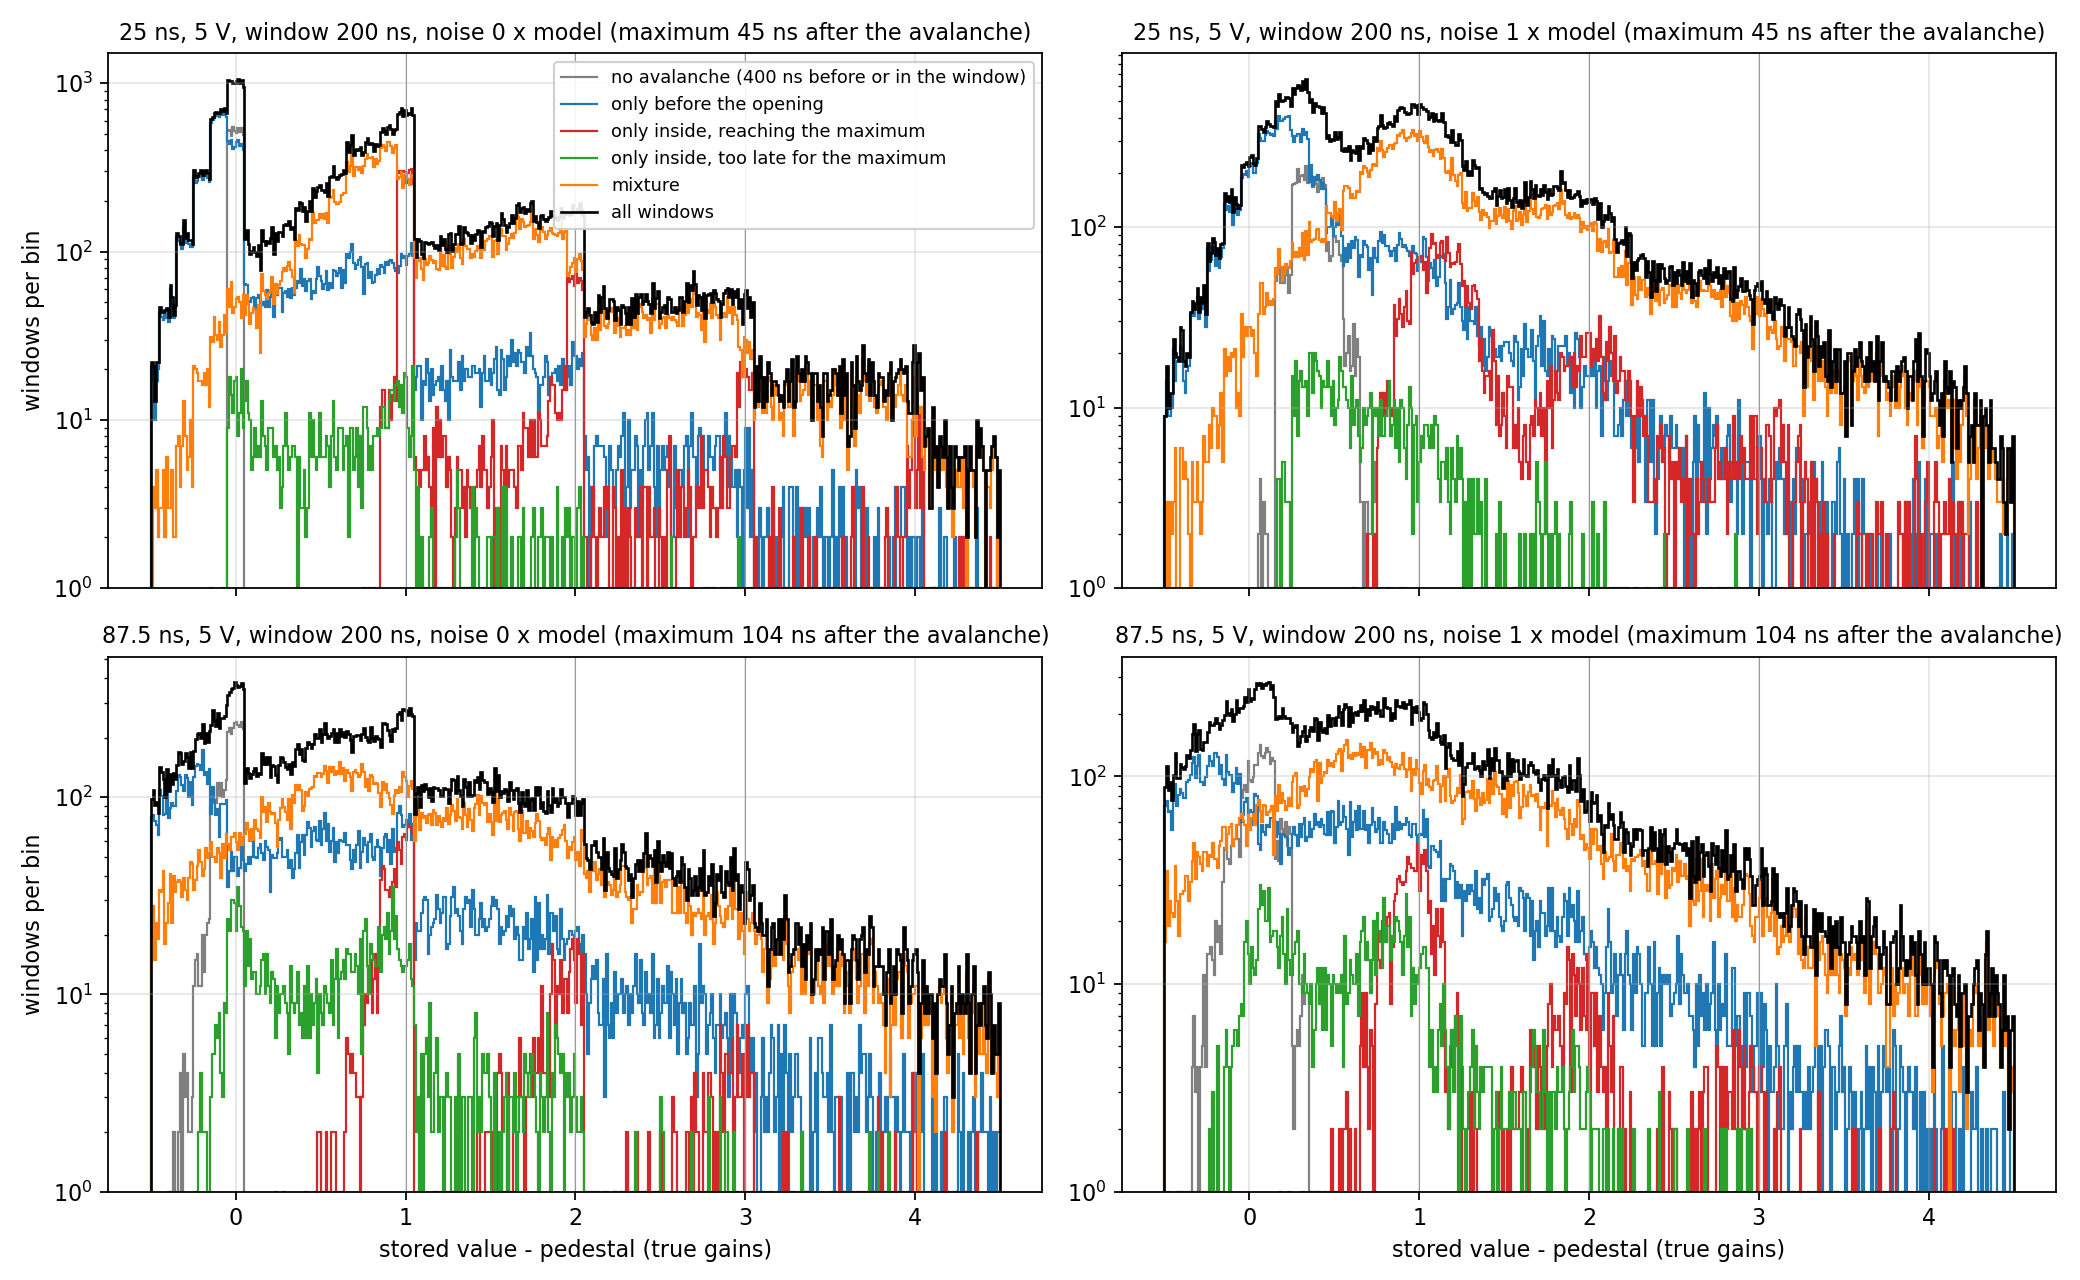
\includegraphics[width=\textwidth]{citiroc_decomposition.png}
\caption{Spectrum of the windows of one channel at 20~$^\circ$C, 5~V and
200~ns, at 25~ns (top) and 87.5~ns (bottom) of peaking time, without
(left) and with (right) the noise of the model, in units of the true gain
above the pedestal, split by the arrival of the avalanches relative to the
window.}
\label{fig:decomposition}
\end{figure}

Only 7\% of the windows contain no avalanche at all, and only 4 to 7\%
contain avalanches that arrived inside the window with nothing before it:
these alone form the clean peaks at one, two and three photoelectrons. A
third of the windows open on the falling tail of an avalanche that fired
before them and store the value of that tail at the opening, anywhere
between zero and one photoelectron, or below the pedestal when the window
opens on the negative lobe that the voltage preamplifier gives after each
pulse. Half of the windows contain an avalanche on top of the tail of an
earlier one and store a value between $n$ and $n+1$ photoelectrons. Without
noise the spectrum is then a series of plateaus ending in sharp edges at
the integer values; with noise the edges are smeared and the peak finder
has no peaks to find. These fractions do not depend on the peaking time:
they are set by the dark rate and by the 100~ns fall of the SiPM pulse,
which the voltage preamplifier passes to the shaper.

\begin{figure}[htbp]
\centering
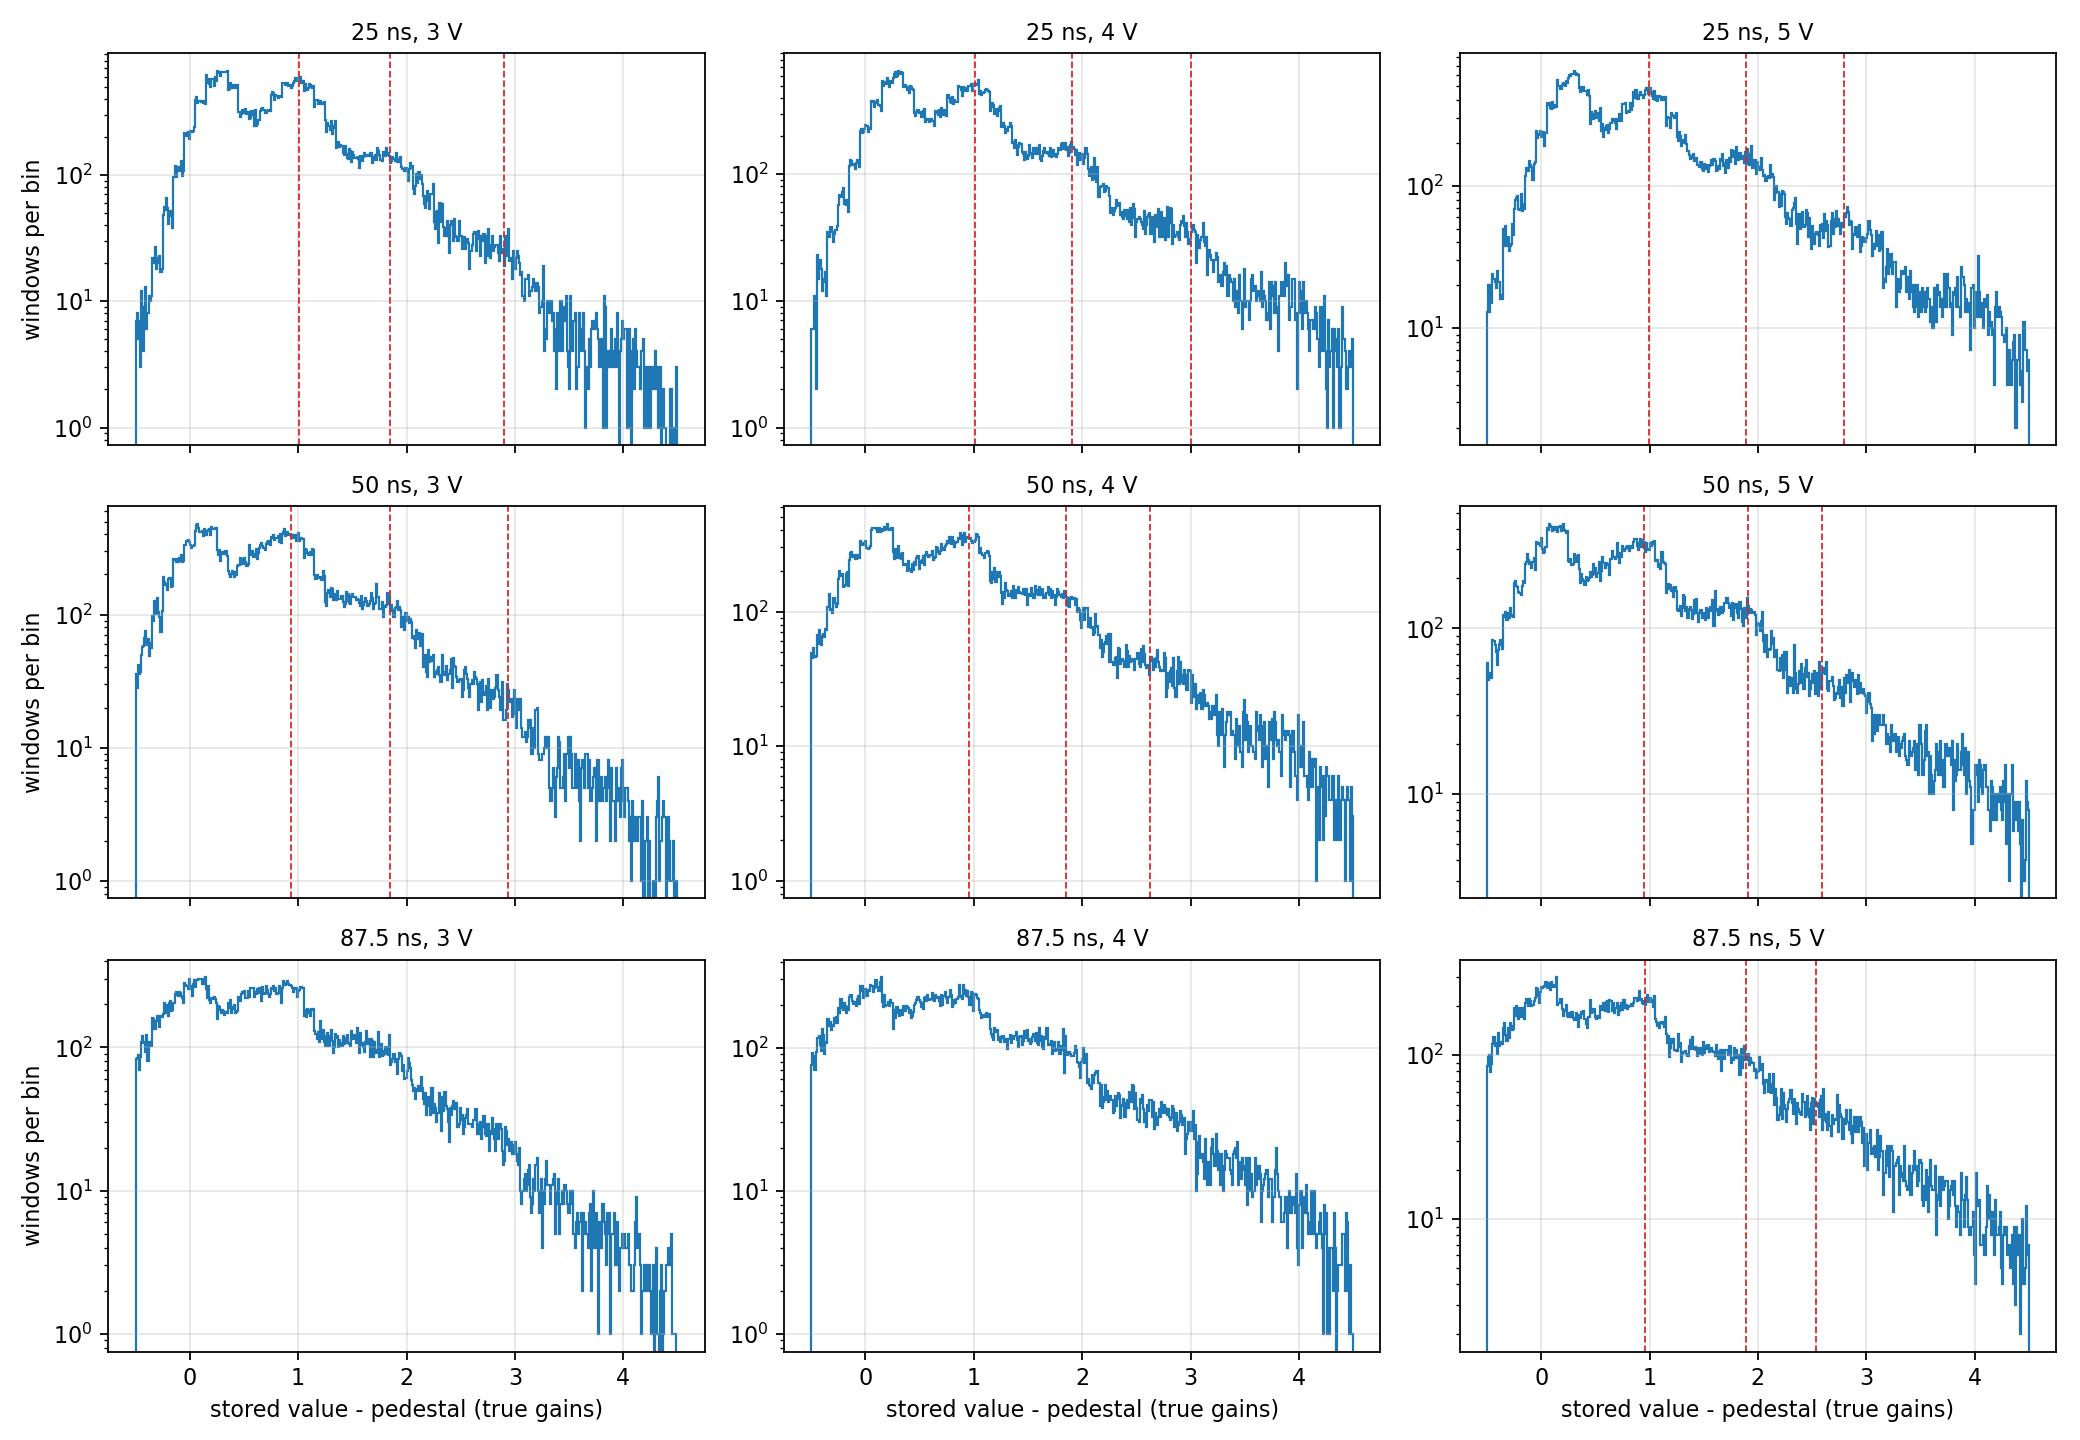
\includegraphics[width=\textwidth]{citiroc_ladders.png}
\caption{Spectrum of the windows of one channel at 20~$^\circ$C at 25, 50
and 87.5~ns (rows) and 3, 4 and 5~V (columns), window 200~ns, noise of the
model; dashed lines: the peaks found by the ladder fit.}
\label{fig:warm_ladders}
\end{figure}

Figure~\ref{fig:warm_ladders} shows the consequence at the three peaking
times and three overvoltages. At 25~ns the ladder fit finds three peaks,
but its gain changes by several per cent between nominally equivalent
samples, between 0.90 and 1.00 of the true one at 5~V; at 50 and 87.5~ns
it ranges from 0.73 to 1.0 or fails, with no stable pattern against the
overvoltage or the noise. The one-photoelectron peak is more robust, with
$k_1 = 1.00$ to 1.01 at 25~ns, but it moves to 0.89 to 0.93 at the longer
peaking times and grows with the window (1.03 at 296~ns, 1.07 at 496~ns),
as the maximum of the noise over a longer window rises. A calibration whose
bias depends on the sample, on the shaping and on the window, and which
the simulation could correct only if it reproduced the dark rate, the
pulse tail and the noise of every channel at the per-cent level, is not
practicable. POLAR-2 reached the same conclusion with this SiPM by direct
waveform analysis: at 25~$^\circ$C the extraction of the
one-photoelectron peak is practically impossible \cite{polar2}.

\section{\texorpdfstring{Cooling the SiPMs to $-3~^\circ$C}{Cooling the SiPMs to -3 C}}
\label{sec:peltier}

A Peltier element in contact with the SiPM board can bring the sensors
below the temperature of the crystal, which stays at room temperature with
its light yield and decay time unchanged (8000~photons per MeV and
0.44~\us for BGO). At $-3~^\circ$C and 5~V the model gives 750~kHz per
channel: 64\% of the windows contain no avalanche, 22\% open on a tail, and
only 4\% contain an avalanche on top of an earlier one, against 51\% at
room temperature. The middle row of Figure~\ref{fig:cold} shows the
result: clean peaks at one, two, three and four photoelectrons, separated
by deep valleys.

\begin{figure}[htbp]
\centering
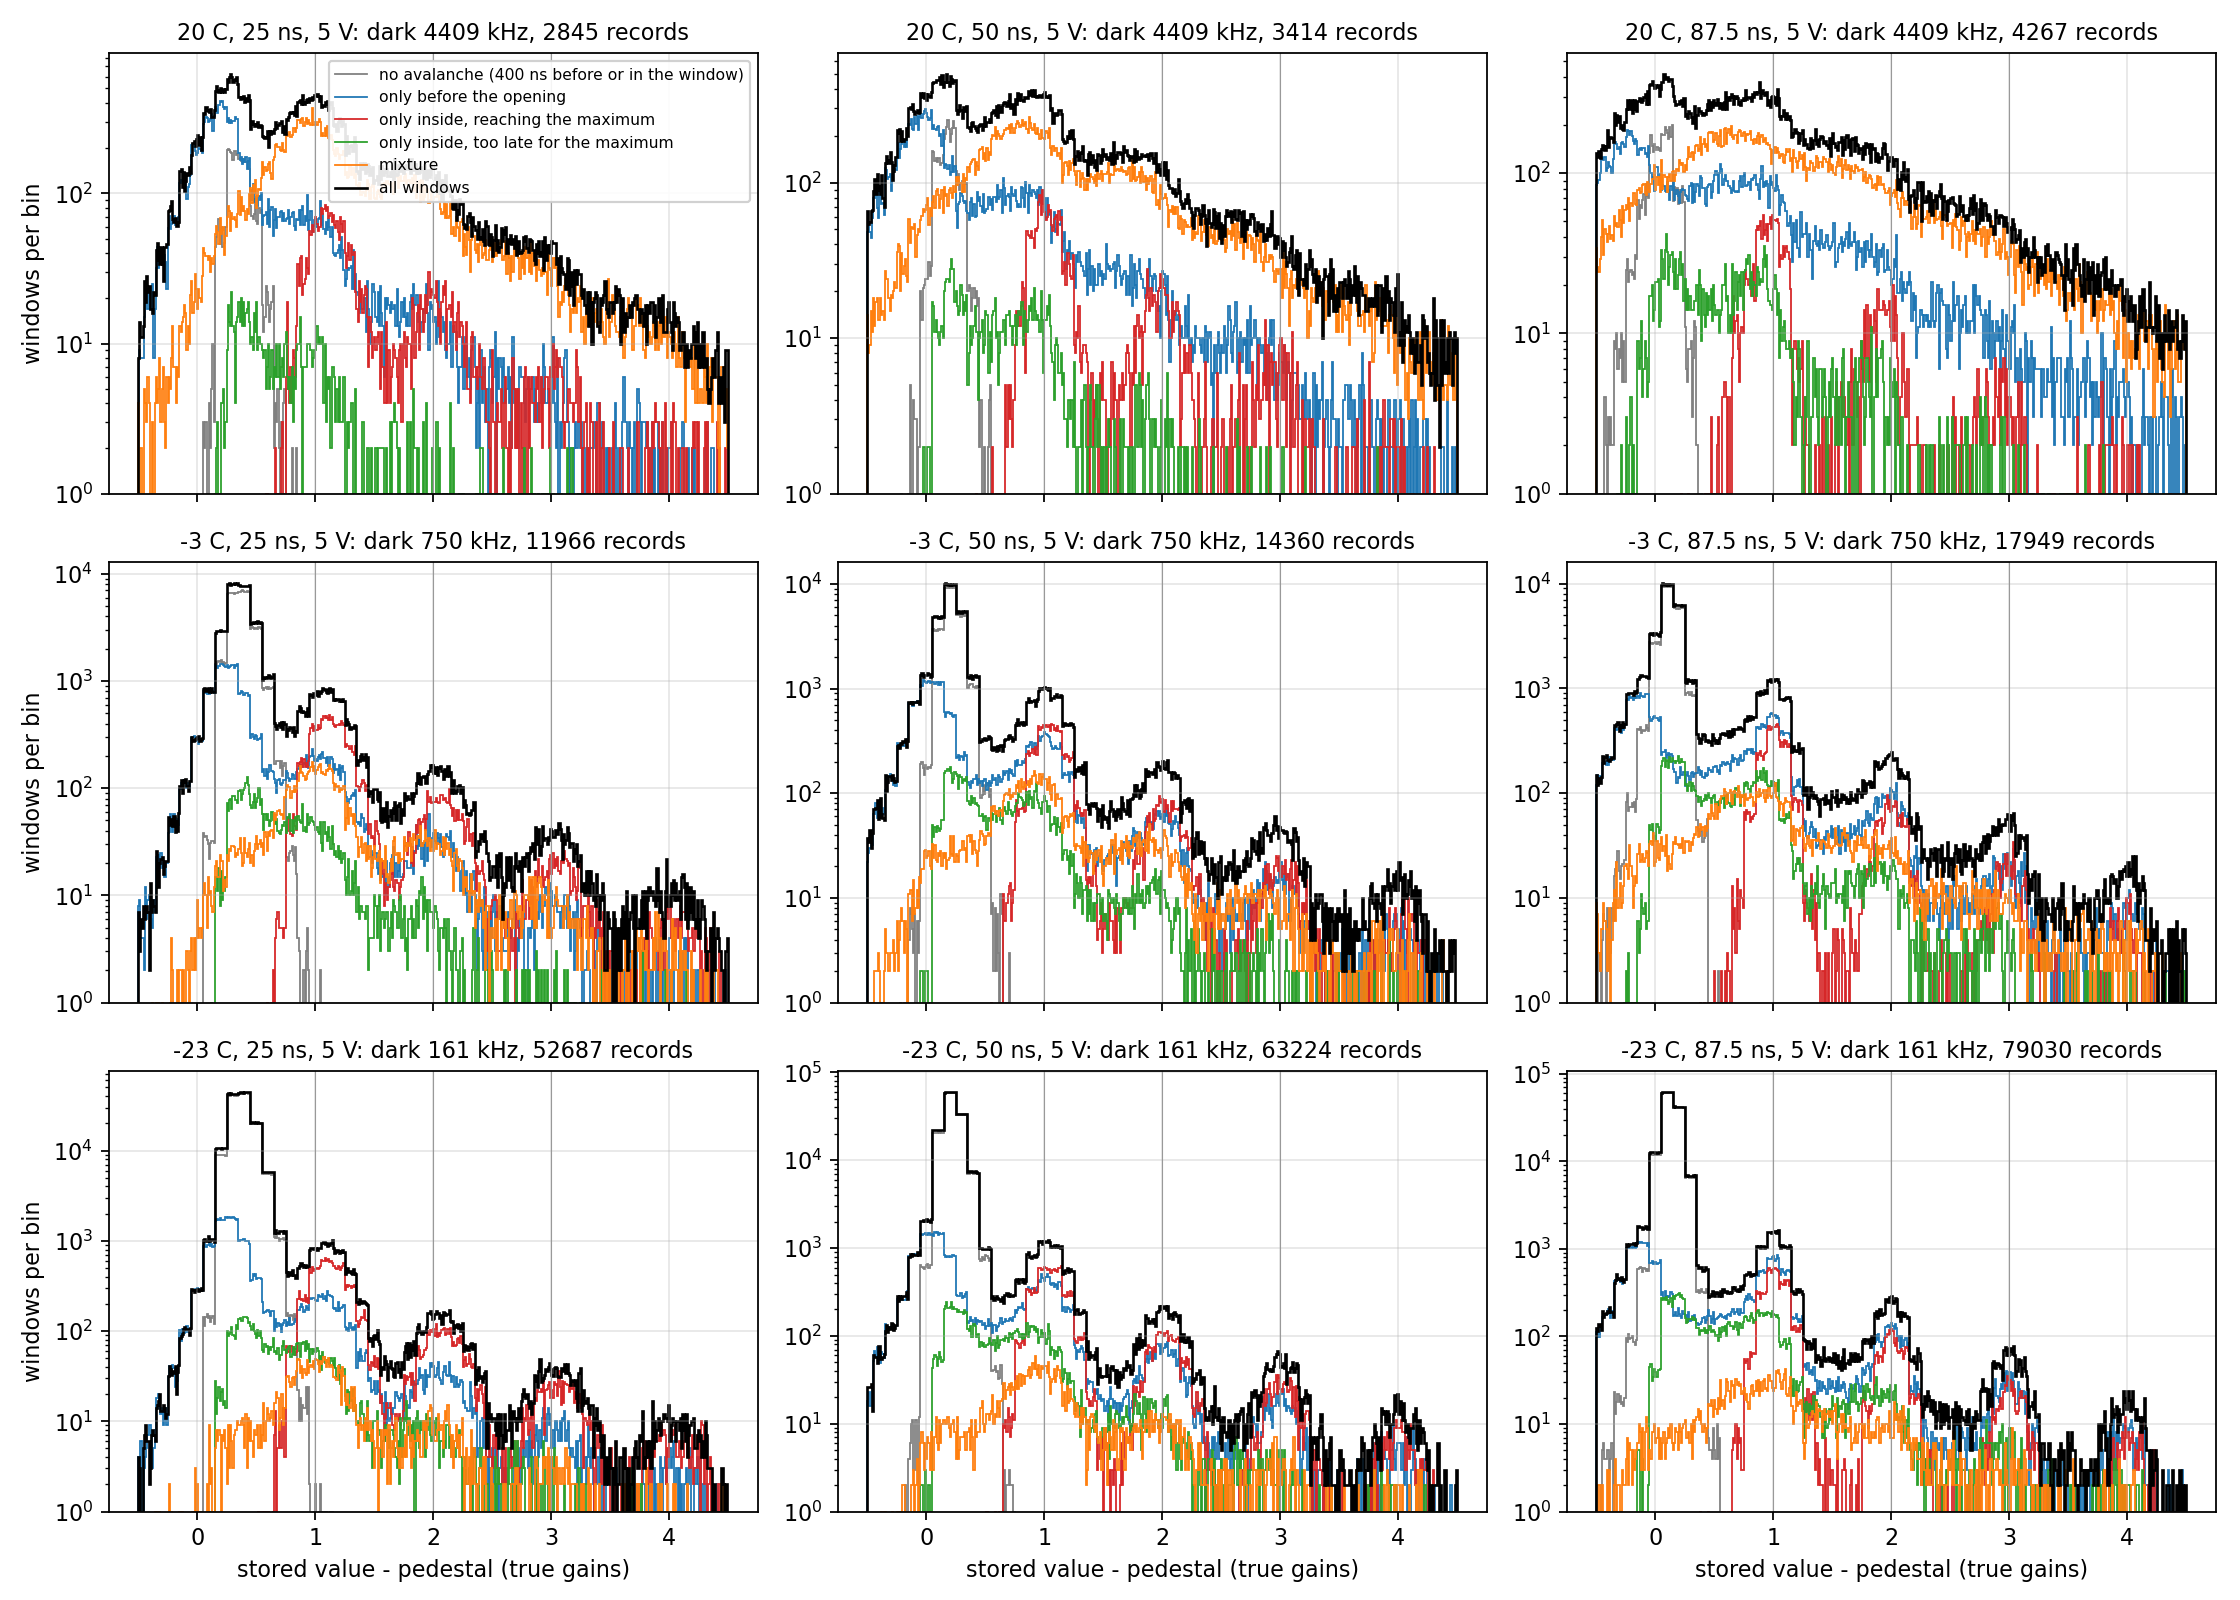
\includegraphics[width=\textwidth]{citiroc_cold.png}
\caption{Spectrum of the windows of one channel at 20, $-3$ and
$-23~^\circ$C (rows) and 25, 50 and 87.5~ns (columns), 5~V of overvoltage
at each temperature, window 200~ns, noise of the model, split by the
arrival of the avalanches as in Figure~\ref{fig:decomposition}. The
number of records grows as the dark rate falls, to keep about 40\,000
windows with an avalanche in each case.}
\label{fig:cold}
\end{figure}

The best peaking time is no longer the shortest. At 25~ns the noise,
0.19~photoelectron rms, raises the maximum stored in an empty window to
about 0.35~photoelectron above the pedestal; since empty windows now
dominate, the zero peak becomes wide and the one-photoelectron fit is
pulled towards it ($k_1 = 0.35$, a failure of the fit rather than a
physical value), although the ladder is still fitted with $k = 0.94$. At
50 and 87.5~ns the noise is smaller and both estimators work: $k = 0.98$
and 0.99, $k_1 = 1.02$ and 1.00 (Figure~\ref{fig:cold_k}). The
calibration of this scenario is therefore made at 87.5~ns of peaking time
on the high gain, the same as the low gain that measures the energy.

\begin{figure}[htbp]
\centering
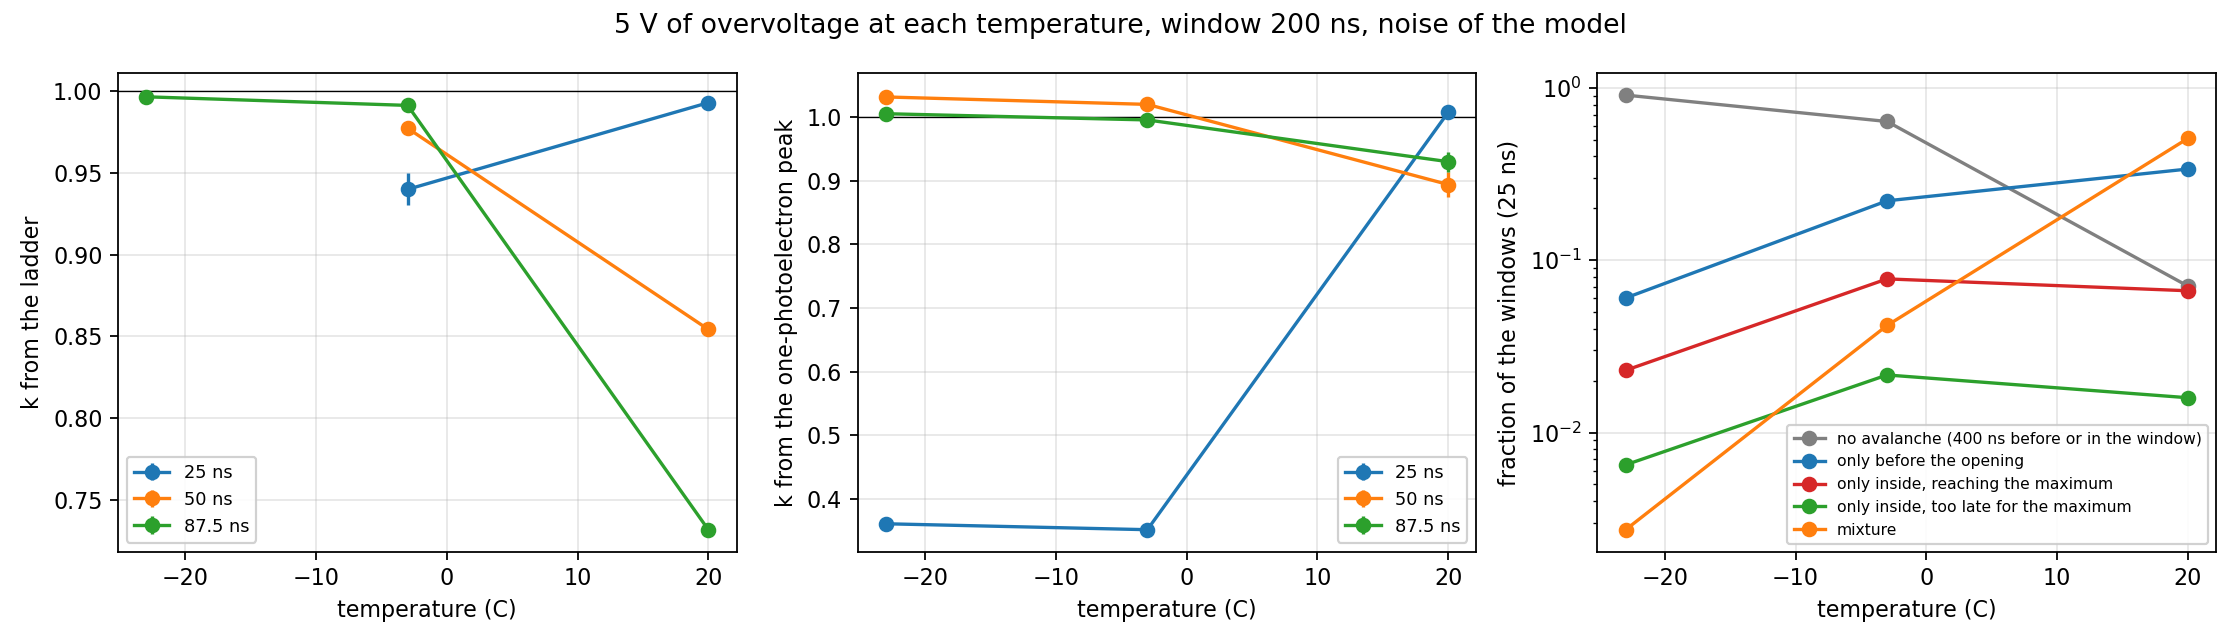
\includegraphics[width=\textwidth]{citiroc_cold_k.png}
\caption{The ratio of the fitted to the true gain from the ladder (left)
and from the one-photoelectron peak (centre) against the temperature, at
5~V and 200~ns, and the fractions of the windows by arrival of their
avalanches at 25~ns (right).}
\label{fig:cold_k}
\end{figure}

\section{\texorpdfstring{Cooling the whole system to $-23~^\circ$C}{Cooling the whole system to -23 C}}
\label{sec:cold}

With the crystal, the SiPMs and the board at 250~K, the model gives
160~kHz per channel at 5~V. Overlapping windows practically disappear
(0.3\%), 91\% of the windows are empty and the ladder extends cleanly to
four photoelectrons (Figure~\ref{fig:cold}, bottom row). At 87.5~ns the
two estimators agree with the true gain to better than 1\%: $k = 0.996$
and $k_1 = 1.005$. At 25 and 50~ns the noise has the effect described for
$-3~^\circ$C, stronger because empty windows are now nine in ten: the
ladder fit fails, and the one-photoelectron peak is usable at 50~ns
($k_1 = 1.03$) but not at 25~ns.

The price is the number of triggers. Only 3\% of the windows of 200~ns
contain an avalanche, so that 40\,000 avalanches per channel require about
1.3~million triggers, against 70\,000 at room temperature and 290\,000 at
$-3~^\circ$C. Every trigger reads the 64 channels at once, and at a
readout rate of a few kHz this is a few minutes per measurement. Since
overlaps are now rare, a longer window would collect more avalanches per
trigger without degrading the spectrum, which is a setting to optimise in
this scenario rather than at room temperature.

The light of BGO at 250~K, its decay time and the fraction of it that the
Citiroc stores are the subject of the note on the cold configuration; for
the calibration only the temperature of the SiPMs matters.

\section{The channels of the array}
\label{sec:channels}

The single-channel results are repeated with the 64 channels of the
array, whose gains are spread by 5\% around the nominal value, in the three
scenarios at their best peaking time: 25~ns at room temperature, 87.5~ns at
$-3$ and $-23~^\circ$C. The number of records gives about 20\,000 windows
with an avalanche per channel: 1423 records of 6.2~\us (36\,000 windows
per channel) at room temperature, 8975 (153\,000) at $-3~^\circ$C and
39\,515 (672\,000) at $-23~^\circ$C. Figure~\ref{fig:scenarios} and
Table~\ref{tab:scenarios} give the result.

\begin{table}[htbp]
\centering
\begin{tabular}{lccc}
\toprule
 & 20~$^\circ$C, 25~ns & $-3~^\circ$C, 87.5~ns & $-23~^\circ$C, 87.5~ns \\
\midrule
dark rate per channel & 4.4~MHz & 750~kHz & 160~kHz \\
ladder fitted & 45 of 64 & 64 of 64 & 64 of 64 \\
$k$, median and rms & $0.923 \pm 0.040$ & $0.993 \pm 0.004$ & $0.994 \pm 0.004$ \\
one-photoelectron peak fitted & 57 of 64 & 64 of 64 & 64 of 64 \\
$k_1$, median and rms & $1.005 \pm 0.017$ & $0.998 \pm 0.002$ & $1.005 \pm 0.003$ \\
\bottomrule
\end{tabular}
\caption{Calibration of the 64 channels in the three scenarios: the
channels in which each estimator gives a gain, and the median and rms over
the channels of its ratio to the true gain. The rms in the cooled
scenarios equals the statistical error of a single channel (0.2 to
0.4\%), so that the estimators add no spread of their own.}
\label{tab:scenarios}
\end{table}

At room temperature the ladder fails in 19 channels and, where it is
fitted, its gain is 8\% low with a spread of 4\% between channels, ten
times the statistical error. The one-photoelectron peak does better, with
a median within 1\% of the true gain and a spread of 1.7\%, but it fails in
seven channels, it cannot be checked against the second and third peaks,
which the ladder does not resolve, and its position depends on the window
and on the noise (Section~\ref{sec:warm}); a correction for these effects
would rest entirely on the simulation. In the two cooled scenarios both
estimators work in every channel, agree with each other and with the true
gain to better than 1\%, and their spread between channels is the
statistical error: the calibration measures the gain of each channel and
nothing else.

\begin{figure}[htbp]
\centering
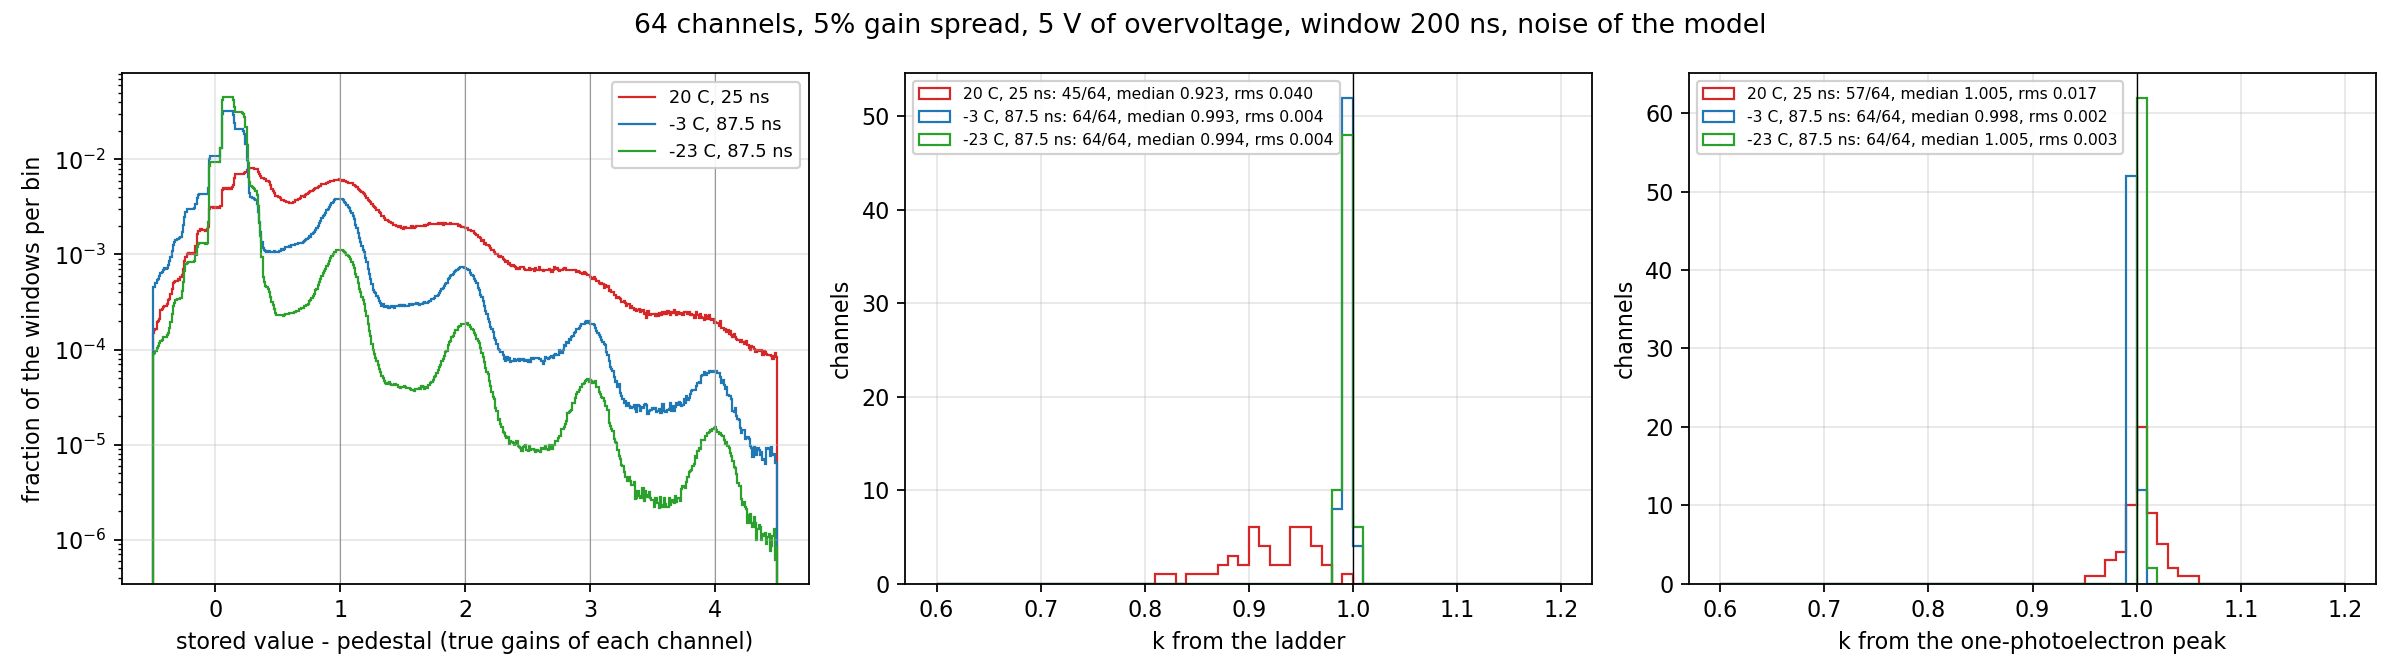
\includegraphics[width=\textwidth]{citiroc_scenarios.png}
\caption{The three scenarios with the 64 channels of the array, gain
spread 5\%, 5~V of overvoltage, window 200~ns: 20~$^\circ$C at 25~ns,
$-3$ and $-23~^\circ$C at 87.5~ns. Left: spectrum of all the channels, each
in units of its own true gain. Centre and right: the ratio of the fitted
to the true gain, channel by channel, from the ladder and from the
one-photoelectron peak.}
\label{fig:scenarios}
\end{figure}

\section{The dark rate against the temperature}
\label{sec:dcr}

The conclusions above rest on the dark-rate law of the model: the rate at
room temperature from the datasheet, divided by two every 9~K. Near room
temperature this is the thermal generation of carriers at levels near the
middle of the gap, a rate proportional to $\exp(-E_a/kT)$ with $E_a$ about
half the band gap of silicon, 0.56~eV, which halves the rate every 9~K at
293~K and every 7~K at 250~K. Liu et al.\ measured the dark rate of the
same SiPM, the S14161-6050HS-04, from 293 to 30~K at 4~V of overvoltage
\cite{liu40k}: it falls from $1.4 \times 10^5$~Hz/mm$^2$ at 293~K to
$10^3$ at 240~K and 20 at 200~K, an activation energy of 0.56~eV between
293 and 240~K, and below about 180~K it stops falling and stays at 1 to
20~Hz/mm$^2$, where the carriers come from band-to-band tunnelling and the
rate depends strongly on the overvoltage and little on the temperature.
The same two regimes were reported for the FBK NUV-HD SiPMs developed for
DarkSide \cite{fbkcryo} and for a Hamamatsu S13360 \cite{naisipm}. For the
calibration, which needs the thermal regime to be suppressed but not
eliminated, only the first matters: tunnelling contributes less than a
kilohertz per channel at any temperature considered here.

Other measurements of the same SiPM between 25 and $-20~^\circ$C give a
slower fall, by a factor of two every 14 to 15~K, an activation energy of
about 0.3~eV \cite{polar2,cattaneo14160}. With that law the dark rate would
be about 1.5~MHz at $-3~^\circ$C and 0.5~MHz at $-23~^\circ$C. At
$-23~^\circ$C this is the rate the model gives at $-3~^\circ$C, where the
calibration already works; the conclusion for the fully cooled scenario
therefore holds for either law, while the margin of the Peltier scenario
depends on which one applies. The rate at the operating temperature is a
direct measurement on the bench (Section~\ref{sec:bench}).

\section{What the bench must measure}
\label{sec:bench}

The simulation fixes the procedure and the expected spectra; four
measurements make them quantitative.

\begin{enumerate}
\item {\bf The pedestal and the noise} of the high-gain path, with the
  SiPMs below breakdown, against the peaking time (menu~1 of the bench
  programme). The noise sets the shaping at which the cooled calibration
  works and the rise of the empty-window peak.
\item {\bf The dark rate} of each channel at the operating temperature and
  overvoltage, from the trigger rate against the threshold (staircase).
\item {\bf The pulse shape} at the output of the slow shaper, with the
  analog probe on an oscilloscope. Its tail decides how many windows open
  on an earlier pulse.
\item {\bf The spectrum with the periodic trigger} in each scenario that
  the set-up allows, at 200~ns and at 87.5~ns of peaking time (and 25~ns at
  room temperature), to compare with Figures~\ref{fig:warm_ladders}
  and~\ref{fig:cold}.
\end{enumerate}

\section{Implementation}
\label{sec:implementation}

{\sloppy
The periodic trigger is the function \texttt{hg\_periodic} of the Citiroc
chain of the simulation (\path{src/frontend/citiroc.jl}), and the two
estimators are \texttt{photoelectron\_ladder} and \texttt{peak\_fit\_window}
of the analysis library (\path{fullsim_analysis/lib/fits.jl}). The
script \path{fullsim_analysis/scripts/citiroc_calib.jl} generates the
dark records of every configuration of this note and writes the spectra,
the decompositions and the fitted gains to
\path{fullsim_analysis/results/calib/citiroc/}; the figures are drawn
from those files by \path{fullsim_analysis/plots/citiroc_calib.py}.
The full calibration of the simulated BGO and CsI(Tl) runs with the
periodic trigger is \path{fullsim_analysis/scripts/calibration.jl} with
the argument \texttt{ptrg}.\par}

\begin{thebibliography}{9}
\bibitem{polar2} S.~Mianowski et al., \emph{Proton irradiation of SiPM
  arrays for POLAR-2}, arXiv:2210.01457 (2022).
\bibitem{liu40k} T.~Liu et al., \emph{Characterization of SiPMs at 40~K
  for neutrino coherent detection based on pure CsI}, Radiat.\ Detect.\
  Technol.\ Methods (2025), arXiv:2509.02041.
\bibitem{fbkcryo} F.~Acerbi et al., \emph{Cryogenic characterization of
  FBK HD near-UV sensitive SiPMs}, arXiv:1610.01915 (2017).
\bibitem{naisipm} H.~Y.~Lee et al., \emph{Scintillation characteristics of a
  NaI(Tl) crystal at low-temperature with silicon photomultiplier},
  arXiv:2110.03306 (2021).
\bibitem{cattaneo14160} P.~W.~Cattaneo et al., \emph{Characterization of
  Hamamatsu 14160 series of silicon photo-multipliers}, arXiv:2006.06258
  (2020).
\end{thebibliography}

\end{document}
